%!TEX program = xelatex

\documentclass[11pt,titlepage]{report}
%!TEX root = main.tex

\usepackage[T1]{fontenc}
\usepackage{lmodern}
\usepackage[svgnames]{xcolor}
\usepackage{fontspec} % XeLaTeX required!
\usepackage{graphicx}
\usepackage{circuitikz}
\usepackage{tikz}
\usepackage{pifont}
\usepackage[some]{background}
\usepackage{xltxtra} 
\usepackage{setspace}
\usepackage[absolute]{textpos}
\usepackage[latin1]{inputenc}
\usepackage[english]{babel}
\usepackage{graphicx}
\usepackage{wrapfig}
\usepackage{fullpage}
\usepackage[margin=1in]{geometry}
\usepackage{float}
\usepackage{url}
\usepackage{multicol}
\usepackage{hyperref}
\usepackage{titlepic}
\usepackage{standalone}
\usepackage{siunitx}
\usepackage{booktabs}
\usepackage{amsmath}
\usepackage{unicode-math}
\usepackage{verbatim}
\usepackage{enumitem}
\usepackage{listings}
\usepackage{multirow}
\usepackage{pgfplots}
\pgfplotsset{compat=1.8}
\usepackage{caption} 
\usepackage[parfill]{parskip}
\usepackage{import}
\usepackage[backend=bibtexu,texencoding=utf8,bibencoding=utf8,style=ieee,sortlocale=en_GB,language=auto]{biblatex}
\usepackage[strict,autostyle]{csquotes}
\usepackage[final]{pdfpages}
\usepackage{subcaption}
\usepackage{ifplatform}
%\captionsetup[table]{skip=10pt}


% Fix for includepdf bug in Mac OS X
\newcommand{\insertpdfpath}[1]{
	\ifwindows
	\newcommand{\insertpdf}[2]{\includepdf[pages=##1]{##2}}
	\else
	\newcommand{\insertpdf}[2]{\includepdf[pages=##1]{#1/##2}}
	\fi
}

%set fonts
\setmainfont[Ligatures=TeX]{Myriad Pro}
\setmathfont{Asana Math}
\setmonofont{Lucida Console}

\usepackage{titlesec, color}
\renewcommand{\familydefault}{\sfdefault} %set font family
\renewcommand{\arraystretch}{1.2} %set table vertical spacing
\setlength\parindent{0pt} %no paragraph indent
\hypersetup{ %setup hyperlinks
    colorlinks,
    citecolor=black,
    filecolor=black,
    linkcolor=black,
    urlcolor=black
}

%redesign chapter headings
\definecolor{gray75}{gray}{0.75}
\newcommand{\chapternumber}{\thechapter}
\newcommand{\hsp}{\hspace{20pt}}
\titleformat{\chapter}[hang]{\Huge\bfseries}{\chapternumber\hsp\textcolor{gray75}{|}\hsp}{0pt}{\Huge\bfseries}

%Redefine appendix headers
\renewcommand{\appendixname}{Appendix}
\renewcommand{\appendixtocname}{Appendices}
\renewcommand{\appendixpagename}{Appendices}

%For code listings
\definecolor{black}{rgb}{0,0,0}
\definecolor{browntags}{rgb}{0.65,0.1,0.1}
\definecolor{bluestrings}{rgb}{0,0,1}
\definecolor{graycomments}{rgb}{0.4,0.4,0.4}
\definecolor{redkeywords}{rgb}{1,0,0}
\definecolor{bluekeywords}{rgb}{0.13,0.13,0.8}
\definecolor{greencomments}{rgb}{0,0.5,0}
\definecolor{redstrings}{rgb}{0.9,0,0}
\definecolor{purpleidentifiers}{rgb}{0.01,0,0.01}


\lstdefinestyle{csharp}{
language=[Sharp]C,
showspaces=false,
showtabs=false,
breaklines=true,
showstringspaces=false,
breakatwhitespace=true,
escapeinside={(*@}{@*)},
columns=fullflexible,
commentstyle=\color{greencomments},
keywordstyle=\color{bluekeywords}\bfseries,
stringstyle=\color{redstrings},
identifierstyle=\color{purpleidentifiers},
basicstyle=\ttfamily\small}

\lstdefinestyle{c}{
language=C,
showspaces=false,
showtabs=false,
breaklines=true,
showstringspaces=false,
breakatwhitespace=true,
escapeinside={(*@}{@*)},
columns=fullflexible,
commentstyle=\color{greencomments},
keywordstyle=\color{bluekeywords}\bfseries,
stringstyle=\color{redstrings},
identifierstyle=\color{purpleidentifiers},
}

\lstdefinestyle{matlab}{
language=Matlab,
showspaces=false,
showtabs=false,
breaklines=true,
showstringspaces=false,
breakatwhitespace=true,
escapeinside={(*@}{@*)},
columns=fullflexible,
commentstyle=\color{greencomments},
keywordstyle=\color{bluekeywords}\bfseries,
stringstyle=\color{redstrings},
identifierstyle=\color{purpleidentifiers}
}

\lstdefinestyle{vhdl}{
language=VHDL,
showspaces=false,
showtabs=false,
breaklines=true,
showstringspaces=false,
breakatwhitespace=true,
escapeinside={(*@}{@*)},
columns=fullflexible,
commentstyle=\color{greencomments},
keywordstyle=\color{bluekeywords}\bfseries,
stringstyle=\color{redstrings},
identifierstyle=\color{purpleidentifiers}
}

\lstdefinestyle{xaml}{
language=XML,
showspaces=false,
showtabs=false,
breaklines=true,
showstringspaces=false,
breakatwhitespace=true,
escapeinside={(*@}{@*)},
columns=fullflexible,
commentstyle=\color{greencomments},
keywordstyle=\color{redkeywords},
stringstyle=\color{bluestrings},
tagstyle=\color{browntags},
morestring=[b]",
  morecomment=[s]{<?}{?>},
  morekeywords={xmlns,version,typex:AsyncRecords,x:Arguments,x:Boolean,x:Byte,x:Char,x:Class,x:ClassAttributes,x:ClassModifier,x:Code,x:ConnectionId,x:Decimal,x:Double,x:FactoryMethod,x:FieldModifier,x:Int16,x:Int32,x:Int64,x:Key,x:Members,x:Name,x:Object,x:Property,x:Shared,x:Single,x:String,x:Subclass,x:SynchronousMode,x:TimeSpan,x:TypeArguments,x:Uid,x:Uri,x:XData,Grid.Column,Grid.ColumnSpan,Click,ClipToBounds,Content,DropDownOpened,FontSize,Foreground,Header,Height,HorizontalAlignment,HorizontalContentAlignment,IsCancel,IsDefault,IsEnabled,IsSelected,Margin,MinHeight,MinWidth,Padding,SnapsToDevicePixels,Target,TextWrapping,Title,VerticalAlignment,VerticalContentAlignment,Width,WindowStartupLocation,Binding,Mode,OneWay,xmlns:x}
}

\lstdefinestyle{matlab}{
language=Matlab,
showspaces=false,
showtabs=false,
breaklines=true,
showstringspaces=false,
breakatwhitespace=true,
escapeinside={(*@}{@*)},
columns=fullflexible,
commentstyle=\color{greencomments},
keywordstyle=\color{bluekeywords}\bfseries,
stringstyle=\color{purpleidentifiers},
identifierstyle=\color{purpleidentifiers}
}

%defaults
\lstset{
basicstyle=\ttfamily\small,
extendedchars=false,
numbers=left,
numberstyle=\ttfamily\tiny,
stepnumber=1,
tabsize=4,
numbersep=5pt
}
\addbibresource{../../library/bibliography.bib}

% Fancy comb dirac, can be ignored for now. For further use.
%
% \usepackage[OT2,T1]{fontenc}
% \newcommand{\sha}{\text{\fontencoding{OT2}\selectfont\char88}}
% \newcommand{\F}[1]{\operatorname{\mathcal{F}}\left\{#1\right\}}
% \begin{equation}
% 	\F{\operatorname{rect}(F_s t) \ast 2F_s \sha(2F_s t)}
% \end{equation}

\begin{document}

\section{Labday 2}
\subsection{Report 8}
The suitabily of four sequences had to be investigated. The four sequences given where:

\begin{equation}
x_1 = [1,-\frac{1}{2},0,0,....]^T \\ 
222
\end{equation}

\begin{equation}
x_2 = [1,-2,0,0,....]^T
\end{equation}
	
\begin{equation}
x_3[n] = \left\{ 
  \begin{array}{l l}
   cos(0.2n) & \quad \textrm{if $0 \leq n \leq N-1 $}\\
    0 & \quad \textrm{if otherwise}
  \end{array} \right.
\end{equation}
 
\begin{equation}
x_4 = sign(randn(N,1))
\end{equation}

For each of this sequences the autocorrelation was calculated and is displayed in Figure~\ref{fig:rep8-autocor}. From this plots we can see that minimum-phase and maximum-phase behave the most like impulses. Impulse behaviour within the autocorrelation means that the signal can better be detected. Thus we can conclude that minimum-phase and maximum-phase are most suited for our purpose. 

\begin{figure}[H]
	\centering
	\begin{subfigure}{0.49\textwidth}
		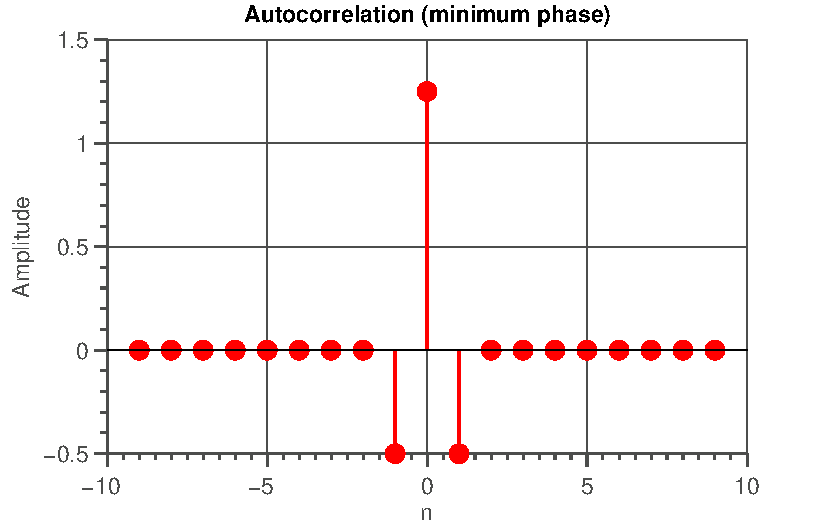
\includegraphics[width=\textwidth]{../../deliverable-7-resources/figures/ass-1/report-8-9-10/report-8/ass-1-report-8-minimum-phase-minimum-phase.pdf}
	\end{subfigure}
	\begin{subfigure}{0.49\textwidth}
		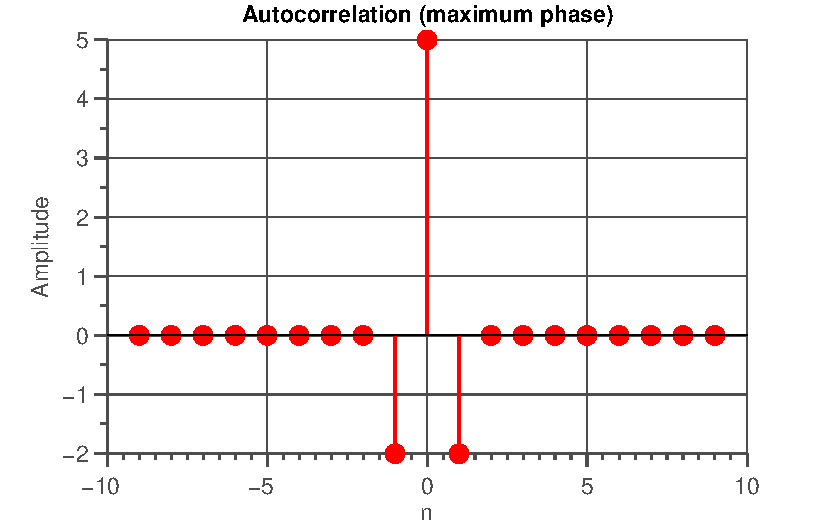
\includegraphics[width=\textwidth]{../../deliverable-7-resources/figures/ass-1/report-8-9-10/report-8/ass-1-report-8-maximum-phase-maximum-phase.pdf}
	\end{subfigure}
	\begin{subfigure}{0.49\textwidth}
		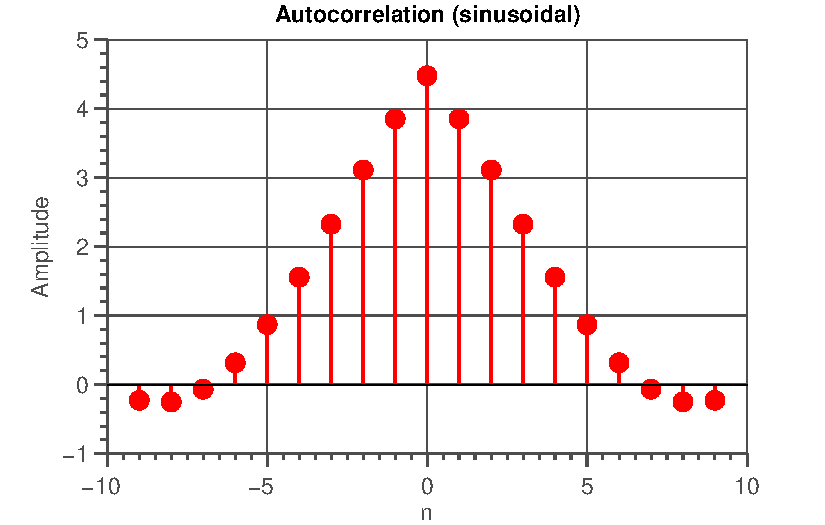
\includegraphics[width=\textwidth]{../../deliverable-7-resources/figures/ass-1/report-8-9-10/report-8/ass-1-report-8-sinusoidal-sinusoidal.pdf}
	\end{subfigure}
	\begin{subfigure}{0.49\textwidth}
		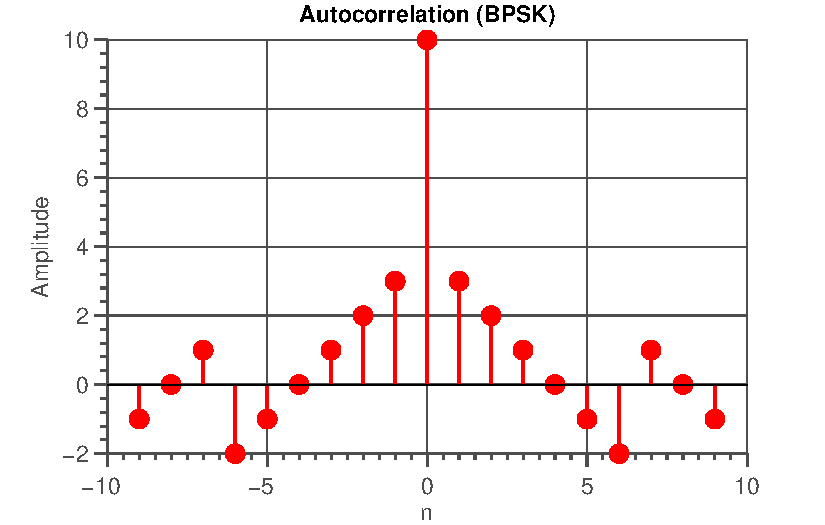
\includegraphics[width=\textwidth]{../../deliverable-7-resources/figures/ass-1/report-8-9-10/report-8/ass-1-report-8-BPSK-BPSK.pdf}
	\end{subfigure}
	\caption{Autocorrelation sequences for each of the tested signals}
	\label{fig:rep8-autocor}
\end{figure}
 

\subsection{Report 9}


\begin{figure}[H]
	\centering
	\begin{subfigure}{0.49\textwidth}
		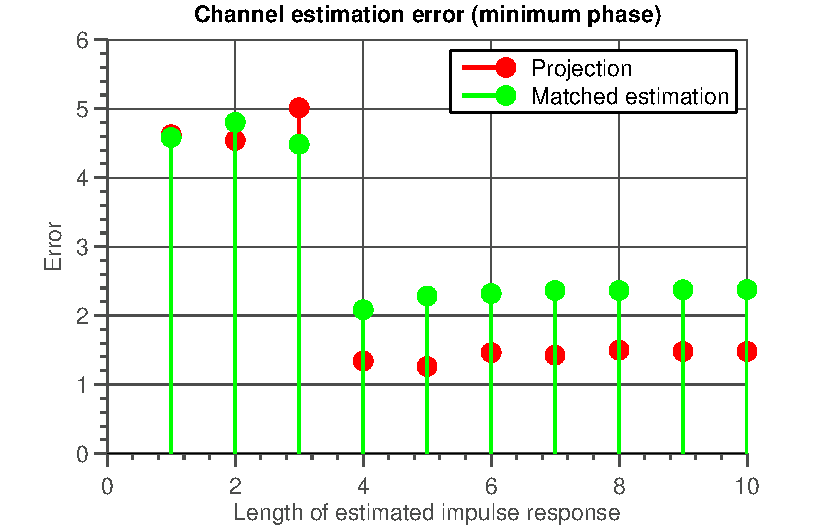
\includegraphics[width=\textwidth]{../../deliverable-7-resources/figures/ass-1/report-8-9-10/report-9-noise-0.5/ass-1-report-9-minimum-phase.pdf}
	\end{subfigure}
	\begin{subfigure}{0.49\textwidth}
		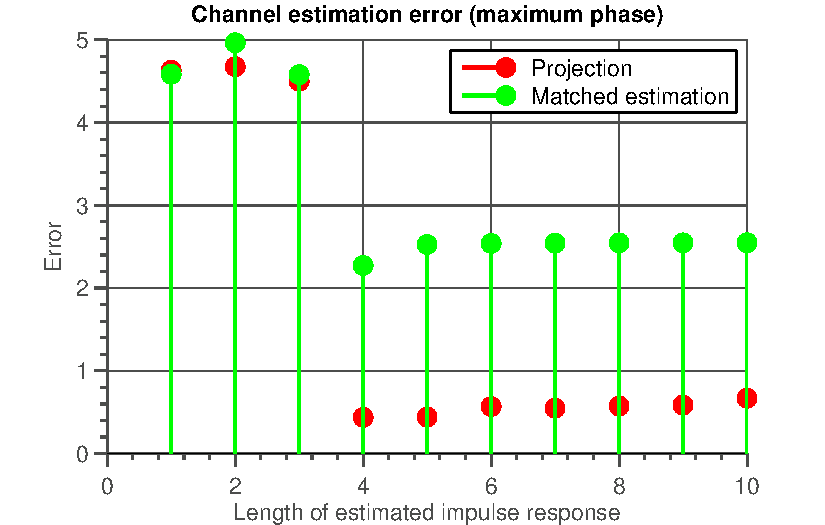
\includegraphics[width=\textwidth]{../../deliverable-7-resources/figures/ass-1/report-8-9-10/report-9-noise-0.5/ass-1-report-9-maximum-phase.pdf}
	\end{subfigure}
	\begin{subfigure}{0.49\textwidth}
		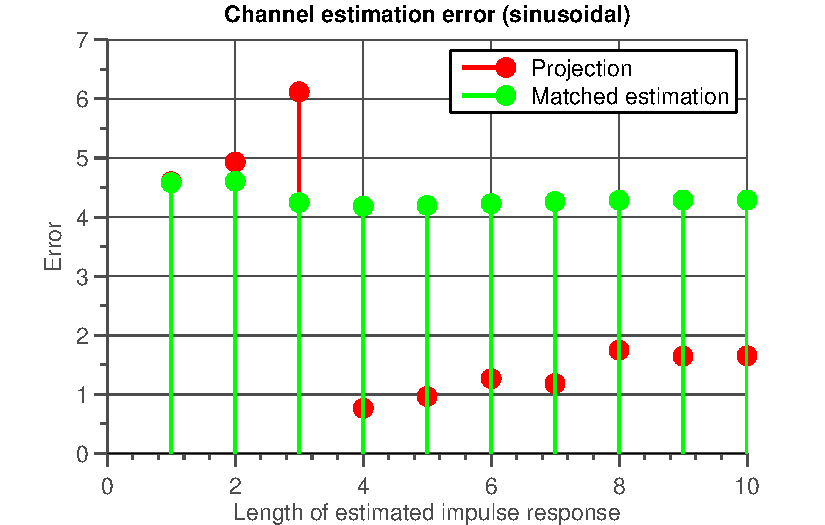
\includegraphics[width=\textwidth]{../../deliverable-7-resources/figures/ass-1/report-8-9-10/report-9-noise-0.5/ass-1-report-9-sinusoidal.pdf}
	\end{subfigure}
	\begin{subfigure}{0.49\textwidth}
		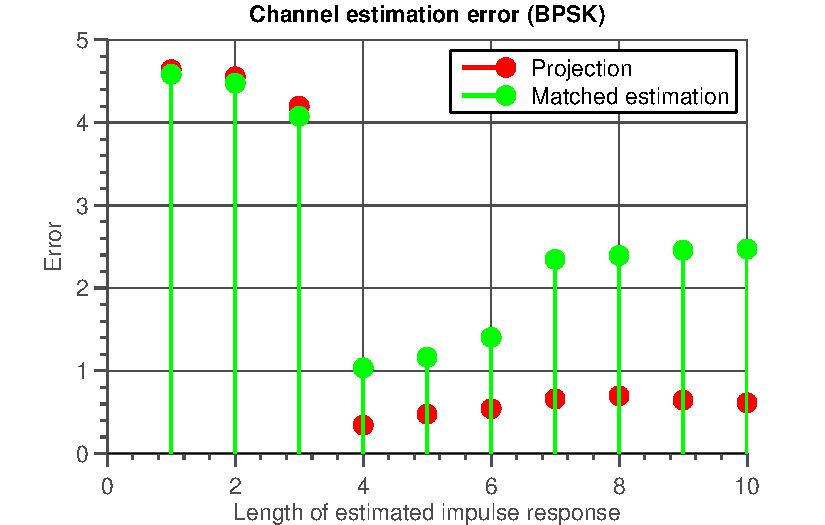
\includegraphics[width=\textwidth]{../../deliverable-7-resources/figures/ass-1/report-8-9-10/report-9-noise-0.5/ass-1-report-9-BPSK.pdf}
	\end{subfigure}
	\caption{The channel estimation error for increasing $\hat{L}$,  with $\sigma = 0.5$ noise}
	\label{fig:rep905}
\end{figure}

The latter Figure~\ref{fig:rep905} shows the channel estimation with $\sigma = 0.5$. We see that the projection estimation method gives better results for $\hat{L} \ge L = 4$. This is to be espected since the projection method is supposed to give perfect results in situations without noise and sufficient estimated channel length, where the matched filter sacrifices estimation accuracy for faster performance due to less complex calculations. \\
Now we see the results for $\sigma = 0.1$ in  Figure~\ref{fig:rep901}. We see that both methods give less errors. This the result we expected since less noise was introduced.

\begin{figure}[H]
	\centering
	\begin{subfigure}{0.49\textwidth}
		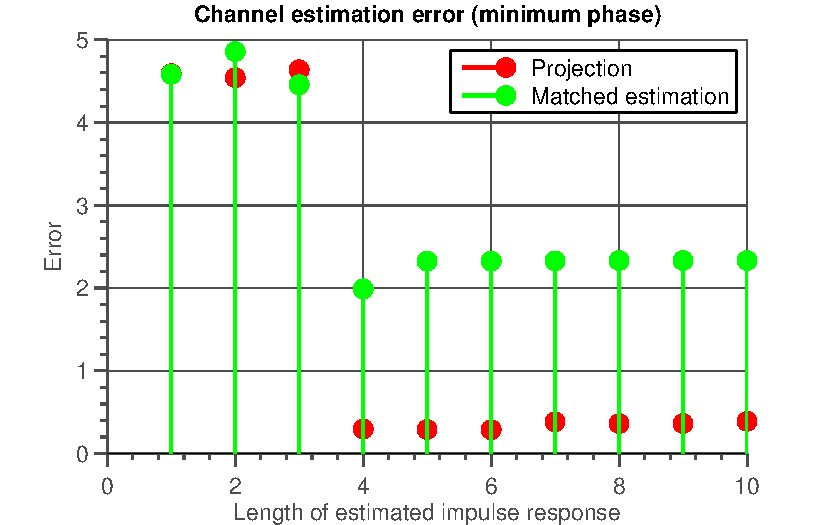
\includegraphics[width=\textwidth]{../../deliverable-7-resources/figures/ass-1/report-8-9-10/report-9-noise-0.1/ass-1-report-9-minimum-phase.pdf}
	\end{subfigure}
	\begin{subfigure}{0.49\textwidth}
		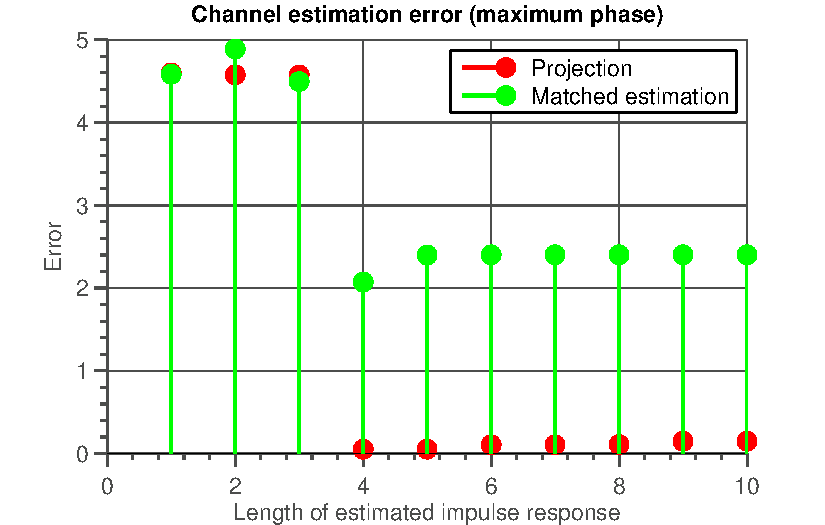
\includegraphics[width=\textwidth]{../../deliverable-7-resources/figures/ass-1/report-8-9-10/report-9-noise-0.1/ass-1-report-9-maximum-phase.pdf}
	\end{subfigure}
	\begin{subfigure}{0.49\textwidth}
		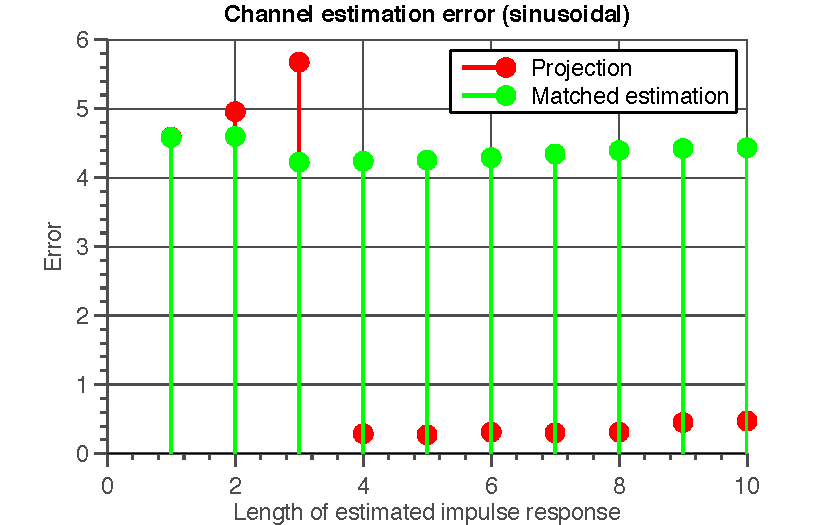
\includegraphics[width=\textwidth]{../../deliverable-7-resources/figures/ass-1/report-8-9-10/report-9-noise-0.1/ass-1-report-9-sinusoidal.pdf}
	\end{subfigure}
	\begin{subfigure}{0.49\textwidth}
		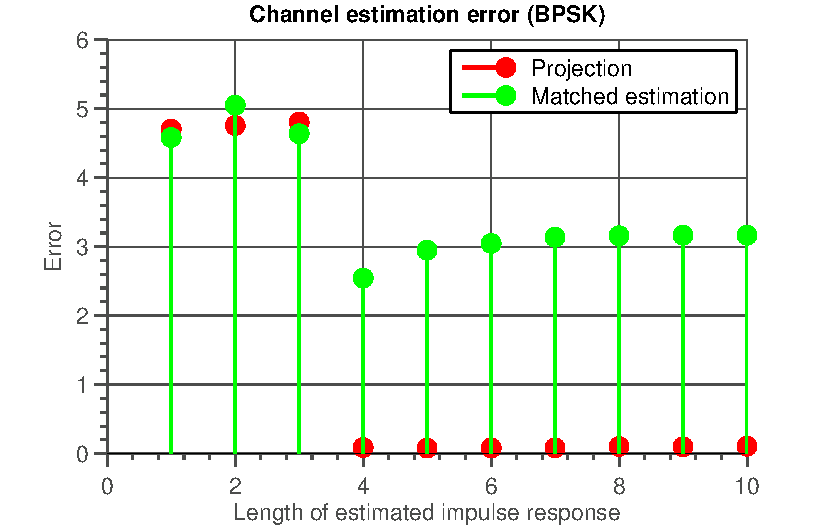
\includegraphics[width=\textwidth]{../../deliverable-7-resources/figures/ass-1/report-8-9-10/report-9-noise-0.1/ass-1-report-9-BPSK.pdf}
	\end{subfigure}
	\caption{The channel estimation error for increasing $\hat{L}$, with $\sigma = 0.1$ noise}
	\label{fig:rep901}
\end{figure}


\subsection{Report 10}
The main idea is to use a training sequence which can always be identified even within surrounding sounds. One of the things that have to be done is giving the training sequence impulse-like autocorrelation behaviour. By doing this the sequence will be well recognizable. Also the crosscorrelation with the surrounding sounds has to be small enough in order to differentiate our signal from surrounding sounds. \\
When choosing a signal length $N_x$ there are pros and cons to be considered. This is the case since a large $N_x$ give a more recognizable sequence, but at the same time increases the time to calculated the position of our car. \\
From the tests we saw that $\hat{L}$ gave sufficiently good results for $\hat{L} = L$. Moreover we want to keep $\hat{L}$ as small as possible since this reduces the complexity of the calculations. Thus we want to keep $\hat{L}$ at $L$.
\end{document}